%Chapter 1 includes Introduction, thesis structure, related work
\chapter{Introduction} %Problem to be solved,  motivation for parallel processing
\section{Motivation and Goals}
As robots continue to be incorporated into human environments, the need for intelligent and high-speed reasoning about the objects around them increases dramatically. At the simplest level, mobile robots need to create a map of their environment for navigation. At a higher level, some robots need to recognize distinct objects in their environment, track object movement, and have some intuitive sense of object geometry that is easily stored and processed. Even more importantly, robots must be able to efficiently generate adaptable models of their environment, or worldview, from sensor data in real time. Many different methods for representing the world have been proposed and implemented, and they will be discussed below in more detail. Like the human brain, the robot should also be able to perform these low level functions with only minimal intervention from higher cognitive functions. Such technology also has potential uses beyond robotics. Applications may include easily modeling indoor environments for interior design concepts, generating 3D tours or maps for various buildings, or low resolution rough mapping of archaeological excavations.\par
This thesis is intended to work towards such a system based on RGB-D cameras, triangle meshes, and the powerful parallel computing capability modern Graphics Processing Units (GPUs) offer. RGB-D cameras like Microsoft's Kinect provide a great low cost solution for capturing 3D environments. Triangle meshes are efficient to store, simple to manipulate and refine, and very versatile. Meshes have the added benefit of being well suited to GPU hardware (which was originally designed for just that purpose). This thesis lays out a robust, high-speed GPU based pipeline that converts raw RGB and depth frames into a 3D textured mesh representation of large planar surfaces in the field of view.
\section{Related Work} %current technology state, Similar systems like kinect fusion
A great variety of methods have been applied to RGB-D camera data in an effort to construct a coherent worldview. Each has advantages and disadvantages.
\subsection{Worldview Storage Models}
\paragraph{Point Cloud Models}
The simplest approach to storing RGB-D data is as a raw point cloud. Each point is stored in a self contained data structure containing at least the point's position and color information. E.g. $$P_i=\{pos_x,pos_y,pos_z,red,green,blue\}$$ This approach allows a complete record of the raw data to be stored very easily, but the size of the data stored will grow very quickly, and simply storing the data linearly results in very slow queries.\par
Nearest neighbor approximations have recently become a popular approach for speeding queries on large point clouds\cite{muja2009fast}. However, achieving reliably fast queries usually requires some form of hierarchical tree structure like K-d trees\cite{nuchter:kdtree} or octrees\cite{octomap}. K-d trees are much more adaptable and usually more efficient in terms of memory storage, but octrees have a significant advantage when it comes to incrementally building a point cloud because points can very easily be inserted into the appropriate octree leaf node with no duplication or restructuring. K-d trees are better suited for compressing point clouds offline.
\paragraph{Voxel Space Models}
%Kinect Fusion, kinfu
Perhaps the most robust and impressive real-time surface reconstruction algorithm to date is Microsoft's Kinect Fusion\cite{newcombe2011kinectfusion,izadi2011kinectfusion}. An open source implementation called KinFu is also available\cite{kinfu}. Kinect Fusion uses a bounded 3D voxel space where each voxel stores the distance to the nearest detected surface  or empty space (the default). Figure~\ref{fig:kinfu_workflow} shows the workflow of the Kinect Fusion system. The point cloud generated by each RGB-D frame is projected into the voxel space and each point updates nearby voxels' distance to nearest surface metric. Implicit surfaces can then be rendered by raycasting through the voxel space and detecting the distance sign crossover point. This results in very high resolution and fidelity reconstructions of the implicit surfaces in the environment. The primary disadvantage of this approach is the workspace size is limited by memory and compute resources which scale with the resolution and dimensions of the voxel space. \par

\begin{figure}[ht]
    \centering
    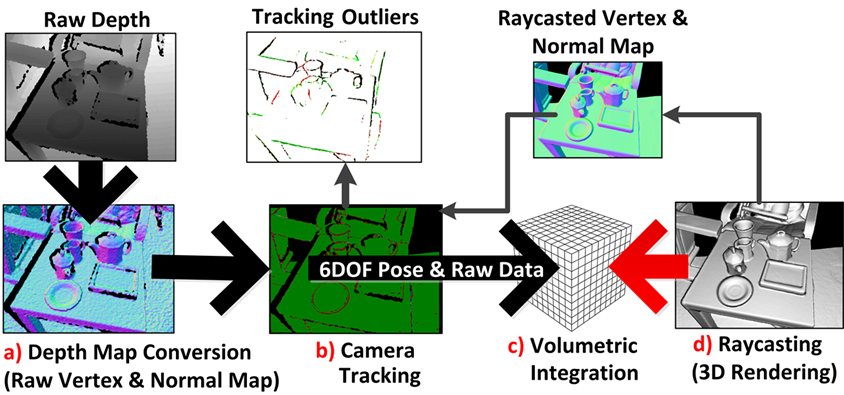
\includegraphics[width=0.8\textwidth]{KinectFusionWorkflow.png}
    \caption{Kinect Fusion Tracking and Reconstruction Pipeline. Reproduced from\cite{izadi2011kinectfusion}}
    \label{fig:kinfu_workflow}
\end{figure}

A spacial extension of this system called Kintinuous was introduced in 2012\cite{whelan2012kintinuous,whelan:odometry}. Kintinuous uses a mobile voxel space which periodically relocates based on camera motion. Voxels that move outside the space are converted to a triangular mesh using a greedy mesh triangulation procedure described by Marton \textit{et al.}\cite{marton:fastreconstruction}.\par
Others have attempted to use sparse voxel octrees (SVOs) to represent larger unbounded spaces using voxels of varying resolution\cite{laine:svo,fastvoxelmaps}. This approach is very amenable to human environments like buildings which are dominated by free space. However, all of these approaches are still limited to storing discrete data points and contain no inherent information about coherent objects or regions.
\paragraph{Point Cloud Offline Processing}
%Poisson Modeling, Mesh generation
Point clouds can also be processed offline to extract surfaces and objects. These systems are not burdened by the strict requirements of real-time computation so they generally can produce more globally optimal solutions than their online counterparts. These systems generally target unordered point clouds. Marton \textit{et al.} proposed an incremental approach to triangulation of noisy point clouds\cite{marton:fastreconstruction}. The approach was amenable to introduction of new registered RGB-D frames by only triangulating points that did not correlate with existing mesh models, but the implementation was far too slow for real-time applications. Ma and Others have introduced a system for planar simplification of dense point clouds using a QuadTree based algorithm\cite{ma2013planar,planesegmentationQTB} and texture maps. This thesis will rely heavily on this innovation. Other approaches worked towards implicit surfaces like parameterized smooth surface fits \cite{hormann2003scattered} or Poisson surfaces\cite{kazhdan2006poisson,bolitho2009parallel}.
\subsection{Real-Time Processing}
A crucial part of this thesis is achieving high speed plane segmentation. Many different researchers have created efficient parallel GPU implementations of common segmentation approaches like Markov Random Fields\cite{arques2006real}, the Potts model\cite{abramov2011real}, parallelized graph-based approaches\cite{wassenberg2009efficient}, seeded region growth (SRG)\cite{pichelparallel}, and region growth based on local smoothness constraints\cite{rabbani2006segmentation}. However, this thesis parallelizes an algorithm by Holz \textit{et al.} \cite{holz2012real} based on clustering in normal space. This approach is superior for application in this thesis because it can readily detect large planes and solve them globally in a very data parallel manner.
\subsection{Additional Resources}
Although this thesis focuses on detecting and representing only planar elements, the envisioned worldview generating pipeline would need several additional components and capabilities to be successful. Additionally, many data processing technologies exist that can improve the quality of the input data through more sophisticated filtering.
\paragraph{RGB-D Filtering}
The Kinect sensor provides its own set of filtering challenges. Khoshelham and Elberink provided a very useful in depth analysis of Kinect accuracy and resolution specifically with indoor mapping applications in mind\cite{khoshelham2012accuracy}. Without some amount of preprocessing and filtering, quantization of the depth data and the fact that resolution and accuracy decrease with increasing distance from the sensor would completely prevent this thesis's pipeline from producing any usable results.\par
This thesis uses bilateral filtering of the depth image\cite{pham2005separable,tomasi1998bilateral}. A simple Gaussian filter is used to smooth local point normals, but other methods exist that could improve results if they could be implemented efficiently in parallel. One such method is adaptively computing filter windows using integral images\cite{holzer2012adaptive}. Kinect data also is notoriously full of holes from washed out areas, shadows and other noise related effects. Some research makes an effort to fill these holes\cite{dakkak2012recovering,spinello2011people,xia2011human}, but this thesis is geared towards progressive improvement of the world model and hopes that any holes will be patched by other viewing angles.
\paragraph{3D SLAM}
This thesis only deals with processing the current frame, but it was designed with an eye towards creating a closed loop system to integrate data from multiple frames. To accomplish this, a Simultaneous Localization and Mapping (SLAM) system will be needed. SLAM has been practically implemented using a Kinect using a GPU \cite{quadrocopterslam,steinbrucker2011real}. Whelan \textit{et al} did fantastic work in comparing multiple SLAM methods combining RGB feature tracking and full point cloud registration algorithms\cite{whelan:odometry}. Other research has evaluated pose graph optimization \cite{Endres} and point-plane alignment\cite{Taguchi} techniques for hand-held 3D sensors like the Kinect.
\paragraph{Mesh Processing and Modification}
One future direction for this work is to incorporate new information into existing meshes through efficient topology changes and resolution modification. The graphics community offers a wide range of insight into these methods, ranging from tracking surfaces through complex topology evolution\cite{bojsen2012tracking}, modeling deformable solids\cite{Sifakis:2007:HSO}, Mesh subdivision and simplification approaches\cite{Puppo:2009:RS}, and texture re-mapping or the effects of image warping\cite{heckbert,heckbert:pixarsurvey,wang:optimaltexture,Oka:RealtimeManipulation,Guo:2008:MOR}.
\section{Thesis Organization} %Outline of thesis
The remainder of this thesis is organized as follows. Chapter~\ref{chap:parallelprogramming} will review some basic precepts of parallel algorithm design, along with specific optimization considerations for programming GPUs with CUDA. Chapter~\ref{chap:approach} will provide an overview of the system design as well as break down the pipeline into sub-modules to be explored in much more detail in Chapter~\ref{chap:implementation}. Finally, Chapters~\ref{chap:analysis} and ~\ref{chap:conclusions} will provide performance analysis, conclusions, and areas of potential improvement for future work.